%%%%%%%%%%%%%%%%%%%%%%%%%%%%%%%%%%%%%%%%%%%%%%%%%%%%%%%%
% Este é um documento que servirá de modelo para
% os relatórios feitos na disciplina Laboratório de Circuitos Lógicos
% 2020-2
%%%%%%%%%%%%%%%%%%%%%%%%%%%%%%%%%%%%%%%%%%%%%%%%%%%%%%%%%

%%%%%%%%%%%%%%%%%%%%%%%%%%%%%%%%%%%%%%%%%%%%%%%%%%%%%%%%%
% Use os diferentes diretórios para colocar os relatórios de cada experimento, deste modo vc consegue manter um histórico e todo material organizado em apenas um local.
% Lembre-se de mudar o Main Document no Menu!!!

\documentclass[12pt]{article}

\usepackage{sbc-template}
\usepackage[brazil,american]{babel}
\usepackage[utf8]{inputenc}

\usepackage{graphicx}
\usepackage{url}
\usepackage{float}
\usepackage{listings}
\usepackage{color}
\usepackage{todonotes}
\usepackage{algorithmic}
\usepackage{algorithm}
\usepackage{hyperref}
\usepackage{amsmath}
\usepackage{graphicx}
\usepackage{array}
\usepackage{mwe}
\usepackage[shortlabels]{enumitem}

\sloppy


\title{Experimento 6\\
Implementação de Circuitos Combinacionais com Multiplexadores}

\author{Matheus Cardoso de Souza, 202033507\\
        Ualiton Ventura da Silva, 202033580\\
        Grupo G42
}

%%%% LEMBRE-SE DE MUDAR O GRUPO NA LINHA ABAIXO!!!!! %%%%%%
\address{Dep. Ciência da Computação -- Universidade de Brasília (UnB)\\
  CIC0231 - Laboratório de Circuitos Lógicos
  \email{matheus-cardoso.mc@aluno.unb.br, 202033580@aluno.unb.br}
}

\begin{document}
\maketitle

\selectlanguage{american}
 \begin{abstract}
   The current report aims to show the elaboration, implementation and analysis
   of logic circuits using multiplexers and decoders as main the main logic
   components. Furthermore, it was explored the use of more advanced tools to
   describe the hardware, using the \emph{SystemVerilog} language for more
   assertive, pratical and scalable representation of complex systems.
 \end{abstract}

\selectlanguage{brazil}
 \begin{resumo}
   O presente relatório tem como objetivo a elaboração, implementação e análise
   de circuitos lógicos utilizando-se multiplexadores e decodificadores como os
   principais componentes lógicos. Além disso, foi explorado o uso de
   ferramentas mais avançadas para a descrição de hardware, valendo-se da
   linguagem \emph{SystemVerilog} para uma representação assertiva, prática e
   escalável de sistemas complexos.
 \end{resumo}


\section{Introdução}
\label{sec:Introducao}

Multiplexadores (ou \emph{mux}) são circuitos combinacionais capazes de mapear
$2^{N}$ entradas para apenas $1$ saída, sendo, portanto, conhecidos também como
\emph{seletores de dados}. No caso, quando existem $2^{N}$ dados de entrada, é
requerido um total de $N$ seletores para satisfatoriamente cumprir o mapeamento
$2^{N} \rightarrow 1$.

Na figura~\ref{fig:mux.png} (fonte:~\cite{isc_mod3}) é possível
entender conceitualmente o funcionamento de um multiplexador, e, na
figura~\ref{fig:mux_wiki.png} (fonte:~\cite{wiki_mux}) é possível visualizar com
maiores detalhes a implementação por circuitos lógicos de um multiplexador.

\begin{figure}[H]
    \centering
    \begin{minipage}{0.45\textwidth}
      \centering
      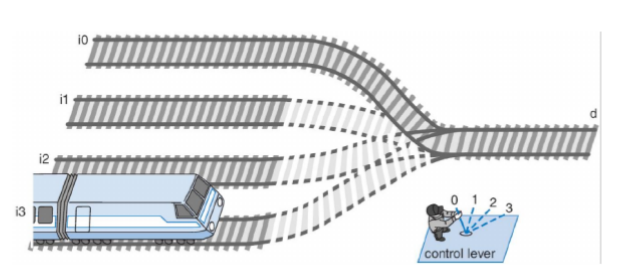
\includegraphics[width=0.9\textwidth]{Exp06/mux.png}
      \caption{Como um multiplexador funciona}\label{fig:mux.png}
    \end{minipage}\hfill
    \begin{minipage}{0.45\textwidth}
      \centering
      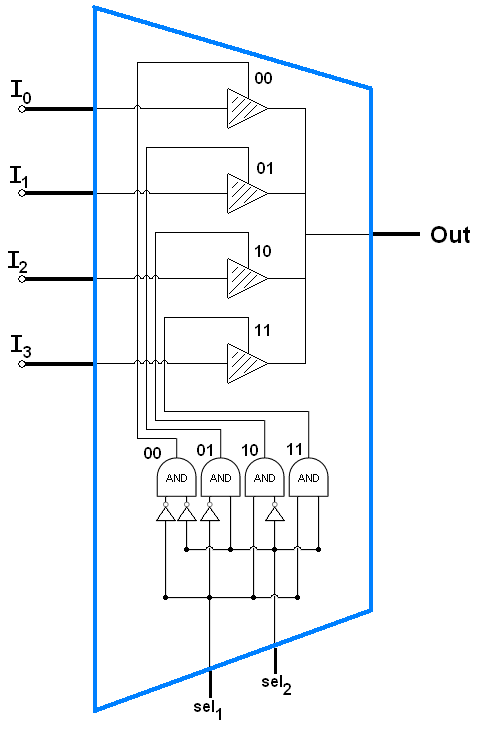
\includegraphics[width=0.5\textwidth]{Exp06/mux_wiki.png}
      \caption{Implementação de um multiplexador}\label{fig:mux_wiki.png}
    \end{minipage}\hfill
\end{figure}

\textbf{***** TODO *****}

\subsection{Objetivos}
\label{sec:Objetivos}

Os textos subsequentes deste presente relatório tem por finalidade a elaboração
de circuitos lógicos para implementação de somadores e funções lógicas
arbitráriass valendo-se de circuitos combinacionais como multiplexadores e
decodificadores. A montagem desses circuitos se dará tanto no nível de
implementação manual dos circuitos e portas lógicas, bem como o uso da linguagem
\emph{SystemVerilog}.

\textbf{***** TODO *****}

\subsection{Materiais}
\label{sec:Materiais}
Em função da natureza do ensino a distância, os presentes experimentos não foram
realizados usando-se materiais e equipamentos físicos, mas sim emulados por meio
do
\href{https://www.intel.com/content/www/us/en/software/programmable/quartus-prime/download.html}{Quartus-II}.

A seguir estão enumerados os materiais utilizados:
\begin{itemize}
    \item Software Quartus-II versão 13.0 SP1
    \item Multiplexadores
    \item Decodificadores
    \item Portas Lógicas \textbf{NOT}, \textbf{Buffer}
    \item \textbf{***** TODO *****}
\end{itemize}

\section{Procedimentos}
\label{sec:Procedimentos}
% \setcounter{subsection}{-1}

Passaremos a apresentar os experimentos requeridos.

% 2.1
\subsection{Elaboração de Somador Completo desenhando o circuito}\label{sec:2.1}

Para a elaboração do somador requerido no enunciado,

\textbf{***** TODO *****}

% 2.2
\subsection{Elaboração de Somador Completo apenas com Verilog}\label{sec:2.2}

\textbf{***** TODO *****}

% 2.3
\subsection{Obtendo as funções booleanas para o decodificador}\label{sec:2.3}

\textbf{***** TODO *****}

\section{Análise dos Resultados}
\label{sec:resultados}

\textbf{***** TODO *****}

\subsection{Análise em \ref{sec:2.1} e \ref{sec:2.2}}\label{sec:analise2.1}

\textbf{***** TODO *****}

\subsection{Análise em \ref{sec:2.3}}\label{sec:analise2.4}

\textbf{***** TODO *****}

\section{Conclusão}
\label{sec:Conclusao}

\textbf{***** TODO *****}

\nocite{*}
\bibliographystyle{sbc}
\bibliography{relatorio}  %Aqui é a definição do arquivo .bib a ser usado pelas referências


\newpage
% Colocar aqui apenas as respostas dos itens da Auto-Avaliação
\section*{Auto-Avaliação}

Respostas:

\textbf{***** TODO *****}

\begin{table}[H]
      \begin{tabular}{|c|c|} \hline
      \textbf{Questão} & \textbf{Resposta}\\
      \hline
      1  & V \\ \hline
      2  & V \\ \hline
      3  & F \\ \hline
      4  & V \\ \hline
      5  & F \\ \hline
      6  & - \\ \hline
      7  & - \\ \hline
      8  & - \\ \hline
      9  & - \\ \hline
      10 & - \\ \hline
      11 & - \\ \hline
      \end{tabular}
\end{table}


\end{document}
